\chapter{Encodings}

First rule: everything in computing is a number. Everything boils down to a
sequence of booleans. When talking about booleans stored on a computer we use
the synonym bit instead. A bit is short for binary digit, which is either 0 or
1. The smallest unit stored on a computer is typically 8 bits, this unit is
called a byte.

Processors understand bytes in groups of different sizes. The representation of
this grouping is different on various processors. When we're using this data, we
understand it fully as a group and don't break it up into different parts. We
call these groups \textbf{primitives}. We would naturally understand a group of
bytes with the most significant byte written to the left writing the next least
significant byte to the right. For instance, a 4 byte primitive is shown below
with the least significant byte being 0-indexed.

\begin{center}
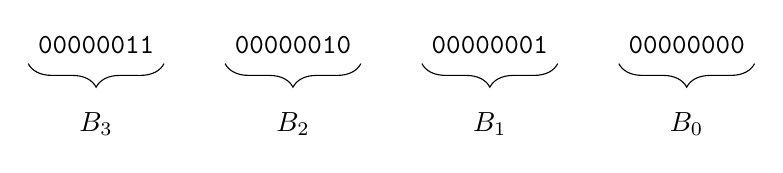
\begin{tikzpicture}
  \node (b3) {\ttfamily 00000011};
  \draw[decorate,decoration={amplitude=3mm,brace,mirror}]
    (b3.south west) -- (b3.south east);
  \node[below of=b3,anchor=center]{$B_3$};

  \node[right of=b3,node distance=2.5cm] (b2) {\ttfamily 00000010};
  \draw[decorate,decoration={amplitude=3mm,brace,mirror}]
    (b2.south west) -- (b2.south east);
  \node[below of=b2,anchor=center]{$B_2$};

  \node[right of=b2,node distance=2.5cm] (b1) {\ttfamily 00000001};
  \draw[decorate,decoration={amplitude=3mm,brace,mirror}]
    (b1.south west) -- (b1.south east);
  \node[below of=b1,anchor=center]{$B_1$};

  \node[right of=b1,node distance=2.5cm] (b0) {\ttfamily 00000000};
  \draw[decorate,decoration={amplitude=3mm,brace,mirror}]
    (b0.south west) -- (b0.south east);
  \node[below of=b0,anchor=center]{$B_0$};
\end{tikzpicture}
\end{center}

\section{Numbers}

Unlike in pure mathematics where we can write numbers up to infinity we are
constrained by bytes on a computer.

\subsection{Naturals}

The values here are exactly like the binary numeral system in
\textbf{Section~\ref{sec:numeral-system-binary}}.

\subsection{Integers}

The most popular integer encoding is \textbf{two's complement}. The sign is
encoded in the \textbf{most significant bit (MSB)}. A value of 0 indicates the
number is positive and the value is the same as the natural number value of the
remaining bits. A value of 1 indicates the number is negative and the value is
obtained from negating all the bits, adding one, and taking the value as the
natural number value of all the bits.

\newpage
\section{Character}

\subsection{ASCII}

{\ttfamily\begin{tabular}{c c}
  \hline
  Value & Meaning \\
  \hline
    0 & \colorbox{gray}{NUL} \\
    1 & \colorbox{gray}{SOH} \\
    2 & \colorbox{gray}{STX} \\
    3 & \colorbox{gray}{ETX} \\
    4 & \colorbox{gray}{EOT} \\
    5 & \colorbox{gray}{ENQ} \\
    6 & \colorbox{gray}{ACK} \\
    7 & \colorbox{gray}{BEL} \\
    8 & \colorbox{gray}{BS} \\
    9 & \colorbox{gray}{HT} \\
   10 & \colorbox{gray}{LF} \\
   11 & \colorbox{gray}{VT} \\
   12 & \colorbox{gray}{FF} \\
   13 & \colorbox{gray}{CR} \\
   14 & \colorbox{gray}{SO} \\
   15 & \colorbox{gray}{SI} \\
   16 & \colorbox{gray}{DLE} \\
   17 & \colorbox{gray}{DC1} \\
   18 & \colorbox{gray}{DC2} \\
   19 & \colorbox{gray}{DC3} \\
   20 & \colorbox{gray}{DC4} \\
   21 & \colorbox{gray}{NAK} \\
   22 & \colorbox{gray}{SYN} \\
   23 & \colorbox{gray}{ETB} \\
   24 & \colorbox{gray}{CAN} \\
   25 & \colorbox{gray}{EM} \\
   26 & \colorbox{gray}{SUB} \\
   27 & \colorbox{gray}{ESC} \\
   28 & \colorbox{gray}{FS} \\
   29 & \colorbox{gray}{GS} \\
   30 & \colorbox{gray}{RS} \\
   31 & \colorbox{gray}{US} \\
\end{tabular}
\quad
\begin{tabular}{c c}
  \hline
  Value & Meaning \\
  \hline
   32 & \colorbox{gray}{SPACE} \\
   33 & ! \\
   34 & " \\
   35 & \# \\
   36 & \$ \\
   37 & \% \\
   38 & \& \\
   39 & ' \\
   40 & ( \\
   41 & ) \\
   42 & * \\
   43 & + \\
   44 & , \\
   45 & - \\
   46 & . \\
   47 & / \\
   48 & 0 \\
   49 & 1 \\
   50 & 2 \\
   51 & 3 \\
   52 & 4 \\
   53 & 5 \\
   54 & 6 \\
   55 & 7 \\
   56 & 8 \\
   57 & 9 \\
   58 & : \\
   59 & ; \\
   60 & < \\
   61 & = \\
   62 & > \\
   63 & ? \\
\end{tabular}
\quad
\begin{tabular}{c c}
  \hline
  Value & Meaning \\
  \hline
   64 & @ \\
   65 & A \\
   66 & B \\
   67 & C \\
   68 & D \\
   69 & E \\
   70 & F \\
   71 & G \\
   72 & H \\
   73 & I \\
   74 & J \\
   75 & K \\
   76 & L \\
   77 & M \\
   78 & N \\
   79 & O \\
   80 & P \\
   81 & Q \\
   82 & R \\
   83 & S \\
   84 & T \\
   85 & U \\
   86 & V \\
   87 & W \\
   88 & X \\
   89 & Y \\
   90 & Z \\
   91 & [ \\
   92 & \textbackslash \\
   93 & ] \\
   94 & \textasciicircum \\
   95 & \_ \\
\end{tabular}
\quad
\begin{tabular}{c c}
  \hline
  Value & Meaning \\
  \hline
   96 & ` \\
   97 & a \\
   98 & b \\
   99 & c \\
  100 & d \\
  101 & e \\
  102 & f \\
  103 & g \\
  104 & h \\
  105 & i \\
  106 & j \\
  107 & k \\
  108 & l \\
  109 & m \\
  110 & n \\
  111 & o \\
  112 & p \\
  113 & q \\
  114 & r \\
  115 & s \\
  116 & t \\
  117 & u \\
  118 & v \\
  119 & w \\
  120 & x \\
  121 & y \\
  122 & z \\
  123 & \{ \\
  124 & | \\
  125 & \} \\
  126 & \textasciitilde \\
  127 & \colorbox{gray}{DEL} \\
\end{tabular}}

\newpage
\section{Data}

\subsection{Base64}

The following is a table of the encoded values:

{\ttfamily\begin{tabular}{c c}
  \hline
  Value & ASCII Character \\
  \hline
   0 & A \\
   1 & B \\
   2 & C \\
   3 & D \\
   4 & E \\
   5 & F \\
   6 & G \\
   7 & H \\
   8 & I \\
   9 & J \\
  10 & K \\
  11 & L \\
  12 & M \\
  13 & N \\
  14 & O \\
  15 & P \\
  16 & Q \\
  17 & R \\
  18 & S \\
  19 & T \\
  20 & U \\
  21 & V \\
  22 & W \\
  23 & X \\
  24 & Y \\
  25 & Z \\
  26 & a \\
  27 & b \\
  28 & c \\
  29 & d \\
  30 & e \\
  31 & f \\
\end{tabular}
\quad
\begin{tabular}{c c}
  \hline
  Value & ASCII Character \\
  \hline
  32 & g \\
  33 & h \\
  34 & i \\
  35 & j \\
  36 & k \\
  37 & l \\
  38 & m \\
  39 & n \\
  40 & o \\
  41 & p \\
  42 & q \\
  43 & r \\
  44 & s \\
  45 & t \\
  46 & u \\
  47 & v \\
  48 & w \\
  49 & x \\
  50 & y \\
  51 & z \\
  52 & 0 \\
  53 & 1 \\
  54 & 2 \\
  55 & 3 \\
  56 & 4 \\
  57 & 5 \\
  58 & 6 \\
  59 & 7 \\
  60 & 8 \\
  61 & 9 \\
  62 & + \\
  63 & / \\
\end{tabular}}
